% !TeX program = xelatex
% !TeX encoding = utf8
% !TeX root = SigSys1_HS22.tex

%% TODO: publish to CTAN
\documentclass[margin=normal]{tex/hsrzf}

%%%%%%%%%%%%%%%%%%%%%%%%%%%%%%%%%%%%%%%%%%%%%%%%%%%
% Packages

%% TODO: publish to CTAN
\usepackage{tex/hsrstud}

%% Language configuration
\usepackage{polyglossia}
\setdefaultlanguage[variant=swiss]{german}

%% License configuration
\usepackage[
    type={CC},
    modifier={by-nc-sa},
    version={4.0},
    lang={german},
]{doclicense}

%other Packages
\usepackage{multicol,multirow}
%amssymb,amsmath,fancybox,graphicx,color,lastpage,
%wrapfig,fancyhdr,hyperref,verbatim,floatflt,
%multicol,multirow,rotating,pdflscape,array,longtable

%%%%%%%%%%%%%%%%%%%%%%%%%%%%%%%%%%%%%%%%%%%%%%%%%%%
% Metadata

\course{Elektrotechnik}
\module{SigSys}
\semester{Herbstsemester 2022}

\authoremail{joel.leirer@ost.ch}
\author{\textsl{Joël Leirer} -- \texttt{\theauthoremail}}

% did someone help you with this work?
\contributors{

}

\title{\texttt{\themodule} Zusammenfassung}
\date{\thesemester}

%%%%%%%%%%%%%%%%%%%%%%%%%%%%%%%%%%%%%%%%%%%%%%%%%%%
% Document

\begin{document}

% use roman numberals for introductiory pages
\pagenumbering{roman}

\maketitle

% \begin{abstract}
% \end{abstract}

% show the names of the people who contributed to this document.
% \section*{Contributors}
% \thecontributors

\section*{Lizenz}
\doclicenseThis
\clearpage
\tableofcontents

% actual content
\clearpage
\setcounter{page}{1}
\pagenumbering{arabic}

\section{Signalklassen}
\begin{multicols}{2}
  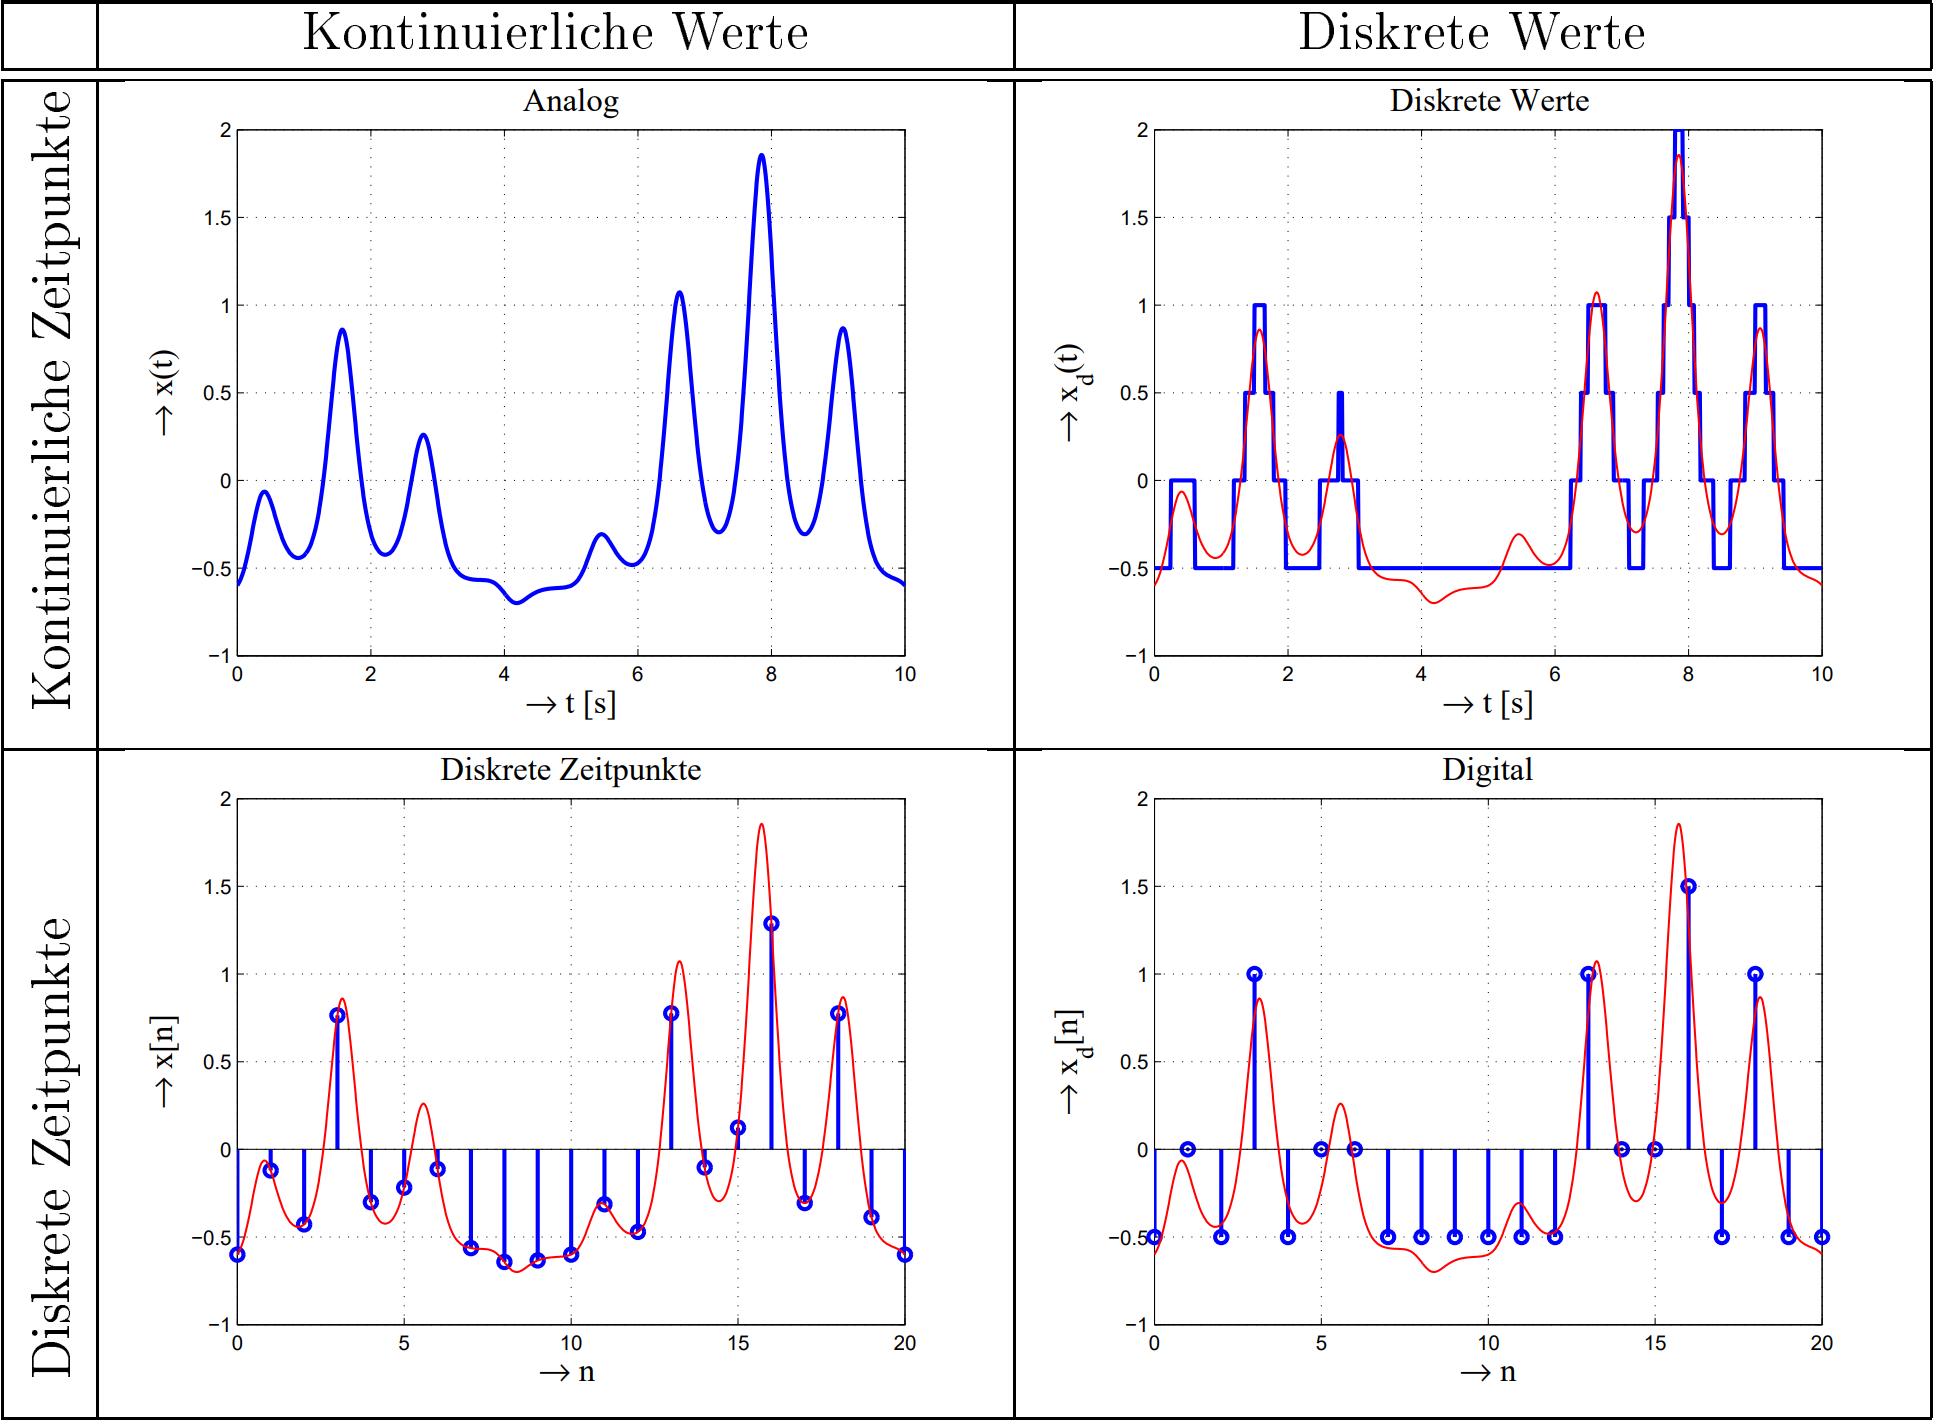
\includegraphics[width = 7cm]{img/Signalklassen.png}
  \subsection{weitere Unterteilungen}
    \begin{tabular}{|c|c|}
    Reellwertig $\mathbb{R}$  &  Complexwertig $\mathbb{C}$ \\
    Eindimensional & Mehrdimensional\\
    Stochastisch & Deterministisch \\
    Energiesignale & Leistungssignal \\
    Analog & Digital \\
    Aperiodisch & Periodisch \\
    \end{tabular}
\end{multicols}
\begin{tabular}{ccc}
  Klasse 1 &
  Klasse 2a &
  Klasse 2b\\
  Energiesiegnal & periodisches Leistungssignal & aperiodisches Leistungssignal\\
  $0 < W_n < \infty $ & $0 < P_n < \infty $ & $0 < P_n < \infty$

\end{tabular}
 
\subsection{Kenngrössen von Signalen}
\begin{tabular}{p{6cm}p{12cm}}
  Linearer Mittelwert 
  \newline \tiny(auch: $ \bar{x}, x_m$)& 
  $X_0 = \frac{1}{T} \int \limits _{-T/2}^{T/2} x(t) dt $ \\
  Quadratischer Mittelwert
  \newline  \tiny(nur Signale Klasse 2a \newline
  Klasse 2b mit: $\lim_{t \to \infty}$) & 
  $X^2 = \frac{1}{T} \int \limits _{-T/2}^{T/2} x^2(t) dt$\\
  Effektivwert \newline \tiny{("Quadratischer Mittelwert", RMS)} &
  $X^2 = \frac{1}{T} \int \limits _{-T/2}^{T/2} \sqrt{x^2(t)} dt $ \\
  Mittelwert n. Ordnung \newline \tiny(nur Signale $\in \mathbb{R}$, Klasse 2a)&
  $X^n = \frac{1}{T} \int \limits _{-T/2} ^{T/2} x^n(t)dt$ \\
  Varianz &
  $Var(x) = \sigma^2 = \frac{1}{T} \int \limits _{-T/2} ^{T/2} (x(t) - X_0)^2 dt$ \\
  Standardabweichung & 
  $\sigma = \sqrt{Var(x)} = \sqrt{X^2 - (X_0)^2}$ \\
\end{tabular} 
 \subsubsection{Die Autokorrelationsfunktion (AKF)}
  $$ \varphi_{xx}(\pm \tau) = \frac{1}{T} \int \limits _{-T/2} ^{T/2} x(t) \cdot x(t- \tau) dt 
  = \frac{1}{T} \int \limits _{-T/2} ^{T/2} x(t + \tau) \cdot x(t)dt$$
  \newline 
\subsubsection*{Eigenschaften:}
%\TODO: Eigenschaften ergänzen
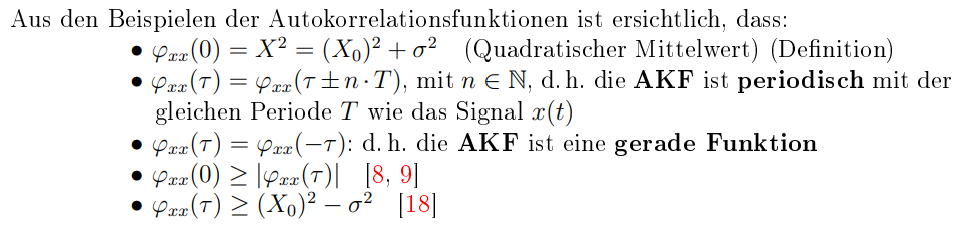
\includegraphics{img/AKF_Prov.png}



\subsection{Wichtige Funktionen}
\begin{tabular}{p{5cm} p{10cm}}
  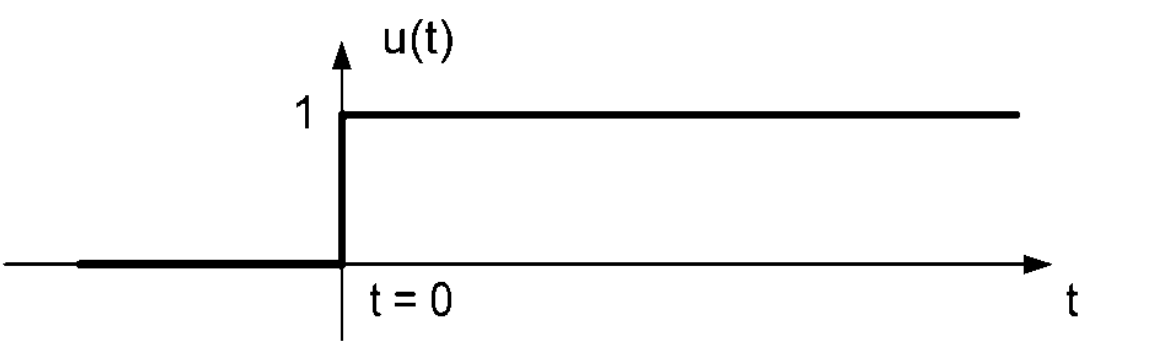
\includegraphics[width = 2.5cm]{img/Sprungfunktion.png} & 
  Sprungfunktion: \newline
  Normierter Einschaltvorgang \newline 
  $ t<0 : u(t) = 0, \ newline
  t \geqslant 0: u(t) = 1 $ \\

  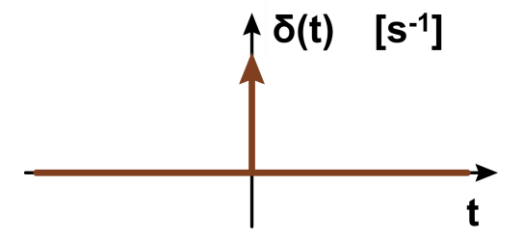
\includegraphics[width = 2.5cm]{img/Impulsfunktion.png} &
  Impulsfunktion = Deltafunktion = \newline 
  Diracimpuls = Delta-Distribution \newline
  Unendlicher kurzer normierter Impuls mit unendlicher Amplitude

  Mathematische Eigenschaften:
$\int\limits _{-\infty} ^{+\infty} f(t) * \delta (t-t_0) dt = f(t_0)$ \newline
$\int\limits _{-\infty} ^{+\infty} f(t) * \delta (t) dt = f(0)$\newline
$\int\limits _{-\infty} ^{+\infty} \delta (t) dt = 1$ \\

\end{tabular}




\section*{Wichtige Werte Vereinfachungen}
\subsubsection*{Integration über Periodendauer}
$\int_T (x \cdot sin(\omega t + \alpha))^2 dt = x^2 \cdot \int_T sin^2(\omega t +\alpha) dt = \frac{x^2}{2}$
$\int_T (x \cdot cos(\omega t+\alpha))^2 dt = x^2 \cdot \int_T cos^2(\omega t+\alpha) dt = \frac{x^2}{2}$
\end{document}
